\documentclass[12pt,letterpaper]{article}
\usepackage[utf8]{inputenc}
\usepackage[spanish, es-tabla]{babel}
\usepackage[version=3]{mhchem}
\usepackage[journal=jacs]{chemstyle}
\usepackage{amsmath}
\usepackage{amsfonts}
\usepackage{amssymb}
\usepackage{makeidx}
\usepackage{xcolor}
\usepackage[stable]{footmisc}
\usepackage[section]{placeins}
%Paquetes necesarios para tablas
\usepackage{longtable}
\usepackage{array}
\usepackage{xtab}
\usepackage{multirow}
\usepackage{colortab}
%Paquete para el manejo de las unidades
\usepackage{siunitx}
\sisetup{mode=text, output-decimal-marker = {,}, per-mode = symbol, qualifier-mode = phrase, qualifier-phrase = { de }, list-units = brackets, range-units = brackets, range-phrase = --}
\DeclareSIUnit[number-unit-product = \;] \atmosphere{atm}
\DeclareSIUnit[number-unit-product = \;] \pound{lb}
\DeclareSIUnit[number-unit-product = \;] \inch{"}
\DeclareSIUnit[number-unit-product = \;] \foot{ft}
\DeclareSIUnit[number-unit-product = \;] \yard{yd}
\DeclareSIUnit[number-unit-product = \;] \mile{mi}
\DeclareSIUnit[number-unit-product = \;] \pint{pt}
\DeclareSIUnit[number-unit-product = \;] \quart{qt}
\DeclareSIUnit[number-unit-product = \;] \flounce{fl-oz}
\DeclareSIUnit[number-unit-product = \;] \ounce{oz}
\DeclareSIUnit[number-unit-product = \;] \degreeFahrenheit{\SIUnitSymbolDegree F}
\DeclareSIUnit[number-unit-product = \;] \degreeRankine{\SIUnitSymbolDegree R}
\DeclareSIUnit[number-unit-product = \;] \usgallon{galón}
\DeclareSIUnit[number-unit-product = \;] \uma{uma}
\DeclareSIUnit[number-unit-product = \;] \ppm{ppm}
\DeclareSIUnit[number-unit-product = \;] \eqg{eq-g}
\DeclareSIUnit[number-unit-product = \;] \normal{\eqg\per\liter\of{solución}}
\DeclareSIUnit[number-unit-product = \;] \molal{\mole\per\kilo\gram\of{solvente}}
\usepackage{cancel}
%Paquetes necesarios para imágenes, pies de página, etc.
\usepackage{graphicx}
\usepackage{lmodern}
\usepackage{fancyhdr}
\usepackage[left=4cm,right=2cm,top=3cm,bottom=3cm]{geometry}

%Instrucción para evitar la indentación
%\setlength\parindent{0pt}
%Paquete para incluir la bibliografía
\usepackage[backend=bibtex,style=chem-acs,biblabel=dot]{biblatex}
\addbibresource{references.bib}

%Formato del título de las secciones

\usepackage{titlesec}
\usepackage{enumitem}
\titleformat*{\section}{\bfseries\large}
\titleformat*{\subsection}{\bfseries\normalsize}

%Creación del ambiente anexos
\usepackage{float}
\floatstyle{plaintop}
\newfloat{anexo}{thp}{anx}
\floatname{anexo}{Anexo}
\restylefloat{anexo}
\restylefloat{figure}

%Modificación del formato de los captions
\usepackage[margin=10pt,labelfont=bf]{caption}

%Paquete para incluir comentarios
\usepackage{todonotes}

%Paquete para incluir hipervínculos
\usepackage[colorlinks=true,
            linkcolor = blue,
            urlcolor  = blue,
            citecolor = black,
            anchorcolor = blue]{hyperref}

%%%%%%%%%%%%%%%%%%%%%%
%Inicio del documento%
%%%%%%%%%%%%%%%%%%%%%%

\begin{document}
\renewcommand{\labelitemi}{$\checkmark$}

\renewcommand{\CancelColor}{\color{red}}

\newcolumntype{L}[1]{>{\raggedright\let\newline\\\arraybackslash}m{#1}}

\newcolumntype{C}[1]{>{\centering\let\newline\\\arraybackslash}m{#1}}

\newcolumntype{R}[1]{>{\raggedleft\let\newline\\\arraybackslash}m{#1}}

\begin{center}

  \begin{figure}
      \vspace{-45mm}
      \centering
      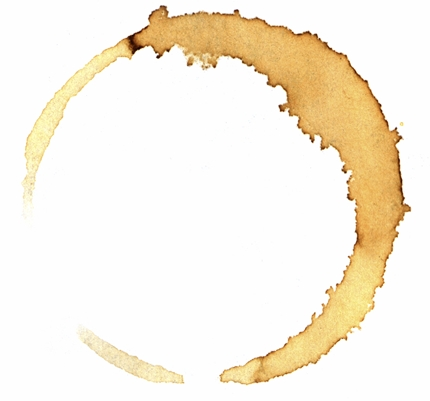
\includegraphics[width=4cm]{./images/cafe-mancha.jpg}
  \end{figure}
  \vspace{-10mm}
  \textbf{\tiny{Apoya tu cafe aqui}} \\
	\vspace{10mm}
  %%%%%%%%%%%%%%%%%%%%%%%%%%%%%%%%%%%%%%
  % Ingresa el mejor titulo que se te ocurra
  %%%%%%%%%%%%%%%%%%%%%%%%%%%%%%%%%%%%%%
	\textbf{\LARGE{Resumen de noticia}}\\
	\vspace{4mm}
		\textbf{\large{Tomás Vera\\
  email: \href{mailto:vtomasv@gmail.com}{vtomasv@gmail.com}  } }\\
	\vspace{3mm}
	\textbf{\large{Universidad de Chile}}\\
	\textbf{\small{CC71T-1 Investigación en Cs. de la Computación.(Métodos,Técnicas,Persp.) }}\\
	\textbf{\large{Profesor: Claudio Gutierrez \\
  email: \href{mailto:cgutierr@dcc.uchile.cl}{cgutierr@dcc.uchile.cl}  } }\\
	\today
\end{center}

%%%%%%%%%%%%%%%%%%%%%%%%%%%%%%%%%%%%%%
% Resumen formal de la noticia
%%%%%%%%%%%%%%%%%%%%%%%%%%%%%%%%%%%%%%
\section*{\centering Resumen}
El resumen es una versión condensada de toda la noticia escrita en apenas 100 a 200 palabras. Para lograr este propósito el resumen debe contener una o dos frases introductorias al tema, es necesario poder indicar un titulo que impulse a leer la noticia, luego debe tener un resumen totalmente imparcial de la noticia para finalizar con un comentario personal sobre la noticia.

%%%%%%%%%%%%%%%%%%%%%%%%%%%%%%%%%%%%%%
% Tu voz sobre el impacto de esta noticia
%%%%%%%%%%%%%%%%%%%%%%%%%%%%%%%%%%%%%%
\section{Opinion}

Esta sección debe incluir tu opinion sobre la noticia, incluyendo las referencia ~\nameref{sec:references}.\autocite{Cooper2009} a esta noticia u otras que ayuden a fundamentar tu opinion.

%%%%%%%%%%%%%%%%%%%%%%%%%%%%%%%%%%%%%%
% Referencias sobre la noticia
%%%%%%%%%%%%%%%%%%%%%%%%%%%%%%%%%%%%%%
\section{Referencias\label{sec:references}}

\printbibliography[heading=none]


\section{Tu opinion es muy importante!}
\begin{figure}
    \centering
    
\includegraphics[width=4cm]{./images/vote.png}
    \captionsetup{justification=centering, singlelinecheck=false}
\end{figure}

\end{document}
